\PassOptionsToPackage{bookmarks={false}}{hyperref}
\documentclass{beamer}
\usepackage{verbatim, mdwlist,tikz,pgfplots}
\usefonttheme{serif}

% This file is a solution template for:

% - Giving a talk on some subject.
% - The talk is between 15min and 45min long.
% - Style is ornate.



% Copyright 2004 by Till Tantau <tantau@users.sourceforge.net>.
%
% In principle, this file can be redistributed and/or modified under
% the terms of the GNU Public License, version 2.
%
% However, this file is supposed to be a template to be modified
% for your own needs. For this reason, if you use this file as a
% template and not specifically distribute it as part of a another
% package/program, I grant the extra permission to freely copy and
% modify this file as you see fit and even to delete this copyright
% notice.


\mode<presentation>
{
  \usetheme{Berkeley}
  % or ...

 % \setbeamercovered{transparent}
  % or whatever (possibly just delete it)
}


%\usepackage[english]{babel}
% or whatever

%\usepackage[latin1]{inputenc}
% or whatever

\usepackage{times}
\usepackage[T1]{fontenc}
% Or whatever. Note that the encoding and the font should match. If T1
% does not look nice, try deleting the line with the fontenc.


\title % (optional, use only with long paper titles)
{Spectral Decomposition of Quantum-Mechanical Operators}

%\subtitle
%{Presentation Subtitle} % (optional)

%\author[Dave Gaebler] % (optional, use only with lots of authors)
%{F.~Author\inst{1} \and S.~Another\inst{2}}
% - Use the \inst{?} command only if the authors have different
%   affiliation.

\institute[Hillsdale College] % (optional, but mostly needed)

\newtheorem{proposition}{Proposition}
\newtheorem{result}{Result}

\newtheorem{question}{Question}[section]
% - Use the \inst command only if there are several affiliations.
% - Keep it simple, no one is interested in your street address.

\date % (optional)
{Tuesday, May 2, 2017\\Daniel Halmrast\\Advisor: Dr. David Gaebler}

%\subject{Talks}
% This is only inserted into the PDF information catalog. Can be left
% out.



% If you have a file called "university-logo-filename.xxx", where xxx
% is a graphic format that can be processed by latex or pdflatex,
% resp., then you can add a logo as follows:

% \pgfdeclareimage[height=0.5cm]{university-logo}{university-logo-filename}
% \logo{\pgfuseimage{university-logo}}



% Delete this, if you do not want the table of contents to pop up at
% the beginning of each subsection:
\AtBeginSubsection[]
{
  \begin{frame}<beamer>{Outline}
    \tableofcontents[currentsection,currentsubsection]
  \end{frame}
}


% If you wish to uncover everything in a step-wise fashion, uncomment
% the following command:

%\beamerdefaultoverlayspecification{<+->}


\begin{document}

\begin{frame}
  \titlepage

\end{frame}

\begin{frame}{Outline}
  \tableofcontents
  % You might wish to add the option [pausesections]
\end{frame}


% Since this a solution template for a generic talk, very little can
% be said about how it should be structured. However, the talk length
% of between 15min and 45min and the theme suggest that you stick to
% the following rules:

% - Exactly two or three sections (other than the summary).
% - At *most* three subsections per section.
% - Talk about 30s to 2min per frame. So there should be between about
%   15 and 30 frames, all told.

\section{Hilbert Space Basics}
\begin{frame}{What Is a Hilbert Space?}
    A \em Hilbert space \em is an inner product space that is complete with
    respect to the induced metric $d(x,y) = \langle x-y, x-y \rangle$.
    \begin{example}
        \begin{enumerate}
        \item $\mathbb{C}^n$ with the inner product 
            $\langle x,y \rangle = x \cdot y$
        \item $L^2(X,\mu)$ with the inner product
            $\langle f,g \rangle = \int_X f\overline{g}d\mu$ (Riesz-Fischer)
        \end{enumerate}
    \end{example}
\end{frame}

\begin{frame}{$L^2(X,\mu)$}
    $L^2(X,\mu)$ is the set of all square-integrable functions from $X$ to
    $\mathbb{C}$ under the equivalence relation
    \[
        f\sim g \iff \int_X |f-g|^2d\mu =0
    \]
    \pause
    \begin{example}
        $L^2(\mathbb{R},dx)$ is the $L^2$ space of functions on the
        real number line.

        \begin{itemize}
            \item The characteristic function $\chi_{[0,1]}(x)$ is a
                square-integrable function with integral 1.
            \item The complex exponential $e^{ikx}$ is not square-integrable on
                the real number line, and is thus not part of
                $L^2(\mathbb{R},dx)$.
        \end{itemize}
    \end{example}
\end{frame}

\begin{frame}{Operators in Hilbert Spaces}
    \begin{itemize}
        \item A \em linear operator \em on a Hilbert space \textbf{H} is a function $T:
        \textbf{H} \to \textbf{H}$ that satisfies
        $T(\alpha x_1 + \beta x_2) = \alpha T(x_1) + \beta T(x_2)$ for $x_1, x_2 \in
        \textbf{H}$.

        \item A linear operator is \em bounded \em if there exists some scalar $C$ such
        that $\forall x\in \textbf{H}: ||T(x)||\leq C||x||$
    \end{itemize}
    \pause
    Fun fact: bounded linear operators are the morphisms in the category
    of Hilbert spaces.
    \pause
    \begin{example}
        \begin{enumerate}
            \item Any matrix $M\in \mathbb{C}^{n\times n}$ is a bounded linear
                operator on $\mathbb{C}^n$.
            \item Given a subspace $M \subset \textbf{H}$, the orthogonal
                projection operator $P_M$ is a bounded linear operator on
                \textbf{H}.
            \item for any essentially bounded function $\phi$ on a measure space
                $(X,\mu)$, the multiplication operator $M_{\phi}$, given by
                $M_{\phi}(f)=\phi f$ is a bounded linear operator on
                $L^2(X,\mu)$.
        \end{enumerate}
    \end{example}
\end{frame}

\begin{frame}{Adjoints and Normality}
    The \em adjoint \em of an operator $A$ on a Hilbert space \textbf{H} is the
    unique operator $A^*$ that satisfies
    \[
        \langle Ax, y \rangle = \langle x, A^*y \rangle
    \]
    for all $x,y$ in \textbf{H}.
    An operator is said to be \em normal \em if it commutes with its adjoint,
    and \em self-adjoint \em if it equals its own adjoint.

    \begin{example}
        \begin{enumerate}
            \item The adjoint of a matrix $M\in \mathbb{C}^{n\times n}$ is the
                conjugate transpose $M^{\dagger}$.
            \item The projection operator $P_M$ is self-adjoint.
            \item The adjoint of the multiplication operator $M_{\phi}$ is
                multiplication by the conjugate $M_{\overline{\phi}}$.
        \end{enumerate}
    \end{example}
\end{frame}

\begin{frame}{The Spectrum of an Operator}

    In finite dimensions, the spectrum of a matrix $M$ is the set of eigenvalues
    for that matrix (i.e. the set of all $\lambda$ such that $(A-\lambda I)x=0$
    for some $x$).

    In infinite dimensions, however, there are more ways to fail invertibility
    than just having a nontrivial kernel.
        \begin{definition}
            The \em spectrum \em of an operator $A$, denoted $\sigma(A)$, is the set of
            all complex numbers $\lambda$ for which the operator $A-\lambda I$ is not
            invertible.
        \end{definition}
\end{frame}

\begin{frame}{The Spectral Partition}
    \begin{question}
        In what ways can $A-\lambda I$ fail to be invertible?
    \end{question}

    \pause

        \begin{enumerate}
            \item $A-\lambda I$ has nontrivial kernel (the \em point spectrum\em).
                \pause
            \item $A-\lambda I$ is not bounded below (the \em approximate point
                spectrum\em).
                \pause
            \item $A-\lambda I$ does not have dense range (the \em compression
                spectrum\em).
        \end{enumerate}
\end{frame}

\begin{frame}{Interpreting the Approximate Point Spectrum}
    For an operator $A-\lambda I$ to \em not \em be bounded below, there must exist some
    sequence $\{h_n\}$ of unit vectors such that 
    \[
        ||(A-\lambda I)h_n|| \to 0
    \]

    \begin{theorem}
        If $A_n$ is a sequence of invertible operators that converge to
        $A-\lambda I$,
        where $A-\lambda I$ is not invertible, then
        $\lambda \in \sigma_{AP}(A)$.
    \end{theorem}

    \begin{theorem}
        $\overline{\sigma_P(A)} \subset \sigma_{AP}(A)$, where 
        $\overline{\sigma_P(A)}$ is the closure of the point spectrum of $A$.
    \end{theorem}
\end{frame}

\begin{frame}{Examples}
    \begin{example}
        In finite dimensions, $\sigma(M) = \sigma_P(M)$. That is, the
        spectrum is entirely a point spectrum.
    \end{example}
    \begin{example}
        The infinite matrix
                $ M = 
                \begin{bmatrix}
                        1 & 0           & \cdots & 0 & \cdots  \\
                        0 & \frac{1}{2} & \cdots & 0 & \cdots  \\
                        \vdots & \vdots & \ddots & 0 & \cdots  \\
                        0 & 0           & 0      & \frac{1}{2^n} & \cdots \\
                        \vdots & \vdots   & \vdots  & \vdots & \ddots
                    \end{bmatrix}
                $
                \\
                has $\sigma_P(M) = \{\frac{1}{2^n}\}$ and
                $\sigma_{AP}(M) = \sigma_P(M) \cup \{0\}$.
    \end{example}
\end{frame}

\begin{frame}{Examples}
    \begin{example}
        Consider the operator $M_x: f(x) \mapsto xf(x)$ on the Hilbert space
        $L^2([0,1],dx)$. 

        \begin{itemize}
            \item For $\lambda \not\in [0,1]$, the operator of multiplication by
                $\frac{1}{x-\lambda}$ inverts $(M_x - \lambda I)$.
            \item For $\lambda \in [0,1]$, the operator has no inverse.
            \item Furthermore, each $\lambda \in [0,1]$ is part of
                $\sigma_{AP}(M_x)$.
        \end{itemize}
            \[
                \{f_n(x)\}_{\lambda} =
            \begin{cases}
                n& \text{if } x\in V_{\frac{1}{n^2}}(\lambda)\\
                0& \text{else}
            \end{cases}
            \]
    \end{example}
\end{frame}

\section{The Spectral Theorem}
\begin{frame}{The Spectral Theorem for Matrices}
    \begin{theorem}[The Spectral Theorem--Finite Dimension]
        Every normal matrix $A$ is unitarily equivalent to a diagonal matrix.
        That is, $A = UDU^*$ for some unitary matrix $U$ and some diagonal
        matrix $D$.
    \end{theorem}
    Here, the unitary matrix has columns equal to the eigenvectors of $A$, and
    the diagonal matrix has the corresponding eigenvalues of $A$.

\end{frame}
\begin{frame}{The Spectral Theorem for Matrices (Cot'd)}
    Alternately,
    \begin{theorem}[The Spectral Theorem--Finite Dimension, Take Two]
        Every normal matrix $A$ is expressable as a linear combination of
        projections onto its eigenspaces. That is,
        \[
            A = \sum_{i=1}^n \lambda_i P_{\lambda_i}
        \]
        where $\{\lambda_i\}$ is the spectrum of $A$, and $P_{\lambda_i}$ is an
        orthogonal projection onto the eigenspace associated with $\lambda_i$.
    \end{theorem}

\end{frame}

\begin{frame}{Measures}
    Extending to infinite dimensions gets tricky, we'll need the idea of a
    measure to continue...
    \pause
    
    A \em measure \em on a space $X$ is a function $\mu: P[X] \to
    \mathbb{R}_+\cup\{\infty\}$
    where:
        \begin{itemize}
            \item $\mu(\emptyset) = 0$
            \item $\mu(A\cup B) = \mu(A) + \mu(B)$ for $A$, $B$ disjoint sets
        \end{itemize}
        \pause
    Intuitively: $\mu$ measures the "weight" of a set.
        \pause

    Practically: $\mu$ allows us to integrate (the Lebesgue Integral).
\end{frame}
\begin{frame}{Measures: Examples}
    \begin{example}
        $X = \mathbb{R}$, and $d\mu = dx$ leads to the standard measure on the
        real number line: $\mu([a,b]) = b-a$. Here, the integral is the standard
        integral
            \[
                \int_{\mathbb{R}}f(x)dx
            \]
    \end{example}
    \pause
    \begin{example}
        $X = \mathbb{N}$, and $d\mu$ is the counting ($\delta$) measure $\mu(S) =
        |S|$. The integral, then, is
        \[
            \int_{\mathbb{N}}f(n)d\mu = \sum_{i=1}^{\infty}f(n)
        \]
    \end{example}

\end{frame}
\begin{frame}{The Spectral Theorem for Operators}
    What happens when we extend to the infinite-dimensional case?

    \begin{theorem}[The Spectral Theorem--Projection-valued Measures]
        Every normal operator $A$ on a Hilbert space \textbf{H} is expressible
        as
        \[
            A = \int_{\sigma(A)} zdE(z)
        \]
        Where $dE$ is a \em projection-valued measure \em on the spectrum of
        $A$.
    \end{theorem}
\end{frame}


\begin{frame}{Examples}
    \begin{example}
        Let $M = 
            \begin{bmatrix}
                \lambda_1 & 0 & \cdots & 0 \\
                0 & \lambda_2 & \cdots & 0 \\
                \vdots & \vdots & \ddots & 0\\
                0 & 0 & 0 & \lambda_n 
            \end{bmatrix}$

            Then, the spectral measure $E(S)$ is the $\delta$-measure on
            $\sigma(M)$ with $E(\lambda_i) = P_{\lambda_i}$, and the spectral
            theorem states that
            \[
                M = \int_{\sigma(M) = \{\lambda_i\}} zdE(z)
                  = \sum_{i=1}^n \lambda_i P_{\lambda_i}
                  \]
            which is a restatement of the familiar spectral theorem.
    \end{example}

\end{frame}

\begin{frame}{Example: Multiplication}
    \begin{example}
        Let $M_x$ be the familiar multiplication operator on $L^2([0,1],dx)$.
        We have seen already that $\sigma(M_x) = \sigma_{AP}(M_x) = [0,1]$.

        The spectral measure $E(S)$ for an interval $S$ is given as $M_{\chi_S}$
        for $\chi_S$ the indicator function on $S$.
    \end{example}
    \[
        M_x = \int_{\sigma(M_x)} zdE(z)
        \]
    \pause
    \begin{question}
        What is $dE(z)$?
    \end{question}
\end{frame}
\begin{frame}{What is $dE(z)$?}
    Motivation: $Ax=\lambda x$, the eigenvalue equation.
    \[
        \begin{aligned}
            M_x f &= \lambda f\\
            xf(x) &= \lambda f(x)\\
            \implies f(x) &= 0 \text{ for } x\not= \lambda
        \end{aligned}
        \]
    \pause
    $f(x) = \delta_{\lambda}(x)$?

    More on this later...
\end{frame}



\begin{frame}{Alternative Approach: Direct Integrals}
    Given a measure space $(X,\mu)$ and a collection of separable Hilbert spaces
    $\{\textbf{H}_{\lambda}\}_{\lambda \in X}$ with a measureability structure,
    the \em direct integral \em 
            \[
                \int_{X}^{\oplus} \textbf{H}_{\lambda} d\mu(\lambda)
            \]
    is the space of equivalence classes of sections $s$ for which
    $||s|| < \infty$ under the norm induced from the inner product
    \[
        \langle s_1, s_2 \rangle = 
        \int_X\langle s_1(\lambda),s_2(\lambda) \rangle d\mu(\lambda)
    \]

\end{frame}

\begin{frame}{The Spectral Theorem--Direct Integral}
    \begin{theorem}
        Given a normal operator $A$, there exists a $\sigma$-finite measure $\mu$
        on $\sigma(A)$ such that A is unitarily equivalent to the multiplication
        operator $M_{\lambda}$ on the direct integral
        \[
            \int_{\sigma(A)}^{\oplus} \textbf{H}_{\lambda} d\mu(\lambda)
        \]
    \end{theorem}

    The $\textbf{H}_{\lambda}$ can be thought of as the "generalized
    eigenspaces" of the operator, and the measure will count their "generalized
    multiplicity". (Remember the $\delta(x)$?)
\end{frame}

\section{Quantum Mechanics}
\begin{frame}{Quantum Lives in a Hilbert Space}
Quantum Mechanics has five basic "axioms" to describe the theory.

    \begin{enumerate}
        \item Associated with each quantum system is a Hilbert space, and
            quantum states are unit vectors in this Hilbert space.
        \item Each classical phase space variable has an associated self-adjoint
            operator known as a quantum observable.
        \item The probability distribution of an observable $\hat{f}$ for a
            quantum state $\psi$ satisfies $\langle f \rangle =
            \langle \psi, \hat{f} \psi \rangle$
        \item If an observable $\hat{f}$ is measured to have a value of
            $\lambda$ for a quantum system with initial state $\psi$, it will
            collapse to a state $\psi '$ satisfying $\hat{f}\psi' = \lambda
            \psi'$
        \item Time evolution is governed by the Schrodinger equation
            \[
                \partial_t \psi - \frac{1}{i\hbar}\hat{H}\psi
            \]
    \end{enumerate}
\end{frame}

\begin{frame}{Quantization of Energy}
    \begin{proposition}
        The quantization of the phase space variables $x$ and $p$ are
        \begin{itemize}
            \item $x \to M_x$
            \item $p \to -i\hbar\frac{d}{dx}$
        \end{itemize}
    \end{proposition}
    \begin{example}
        The standard quantization of kinetic energy uses the identity
        \[
            KE = \frac{p^2}{2m}
        \]
        Which implies that
        \[
            \hat{KE} = \frac{-\hbar^2}{2m}\frac{d^2}{dx^2}
        \]
    \end{example}
\end{frame}
\begin{frame}{The Finite Square Well}

    \begin{center}
    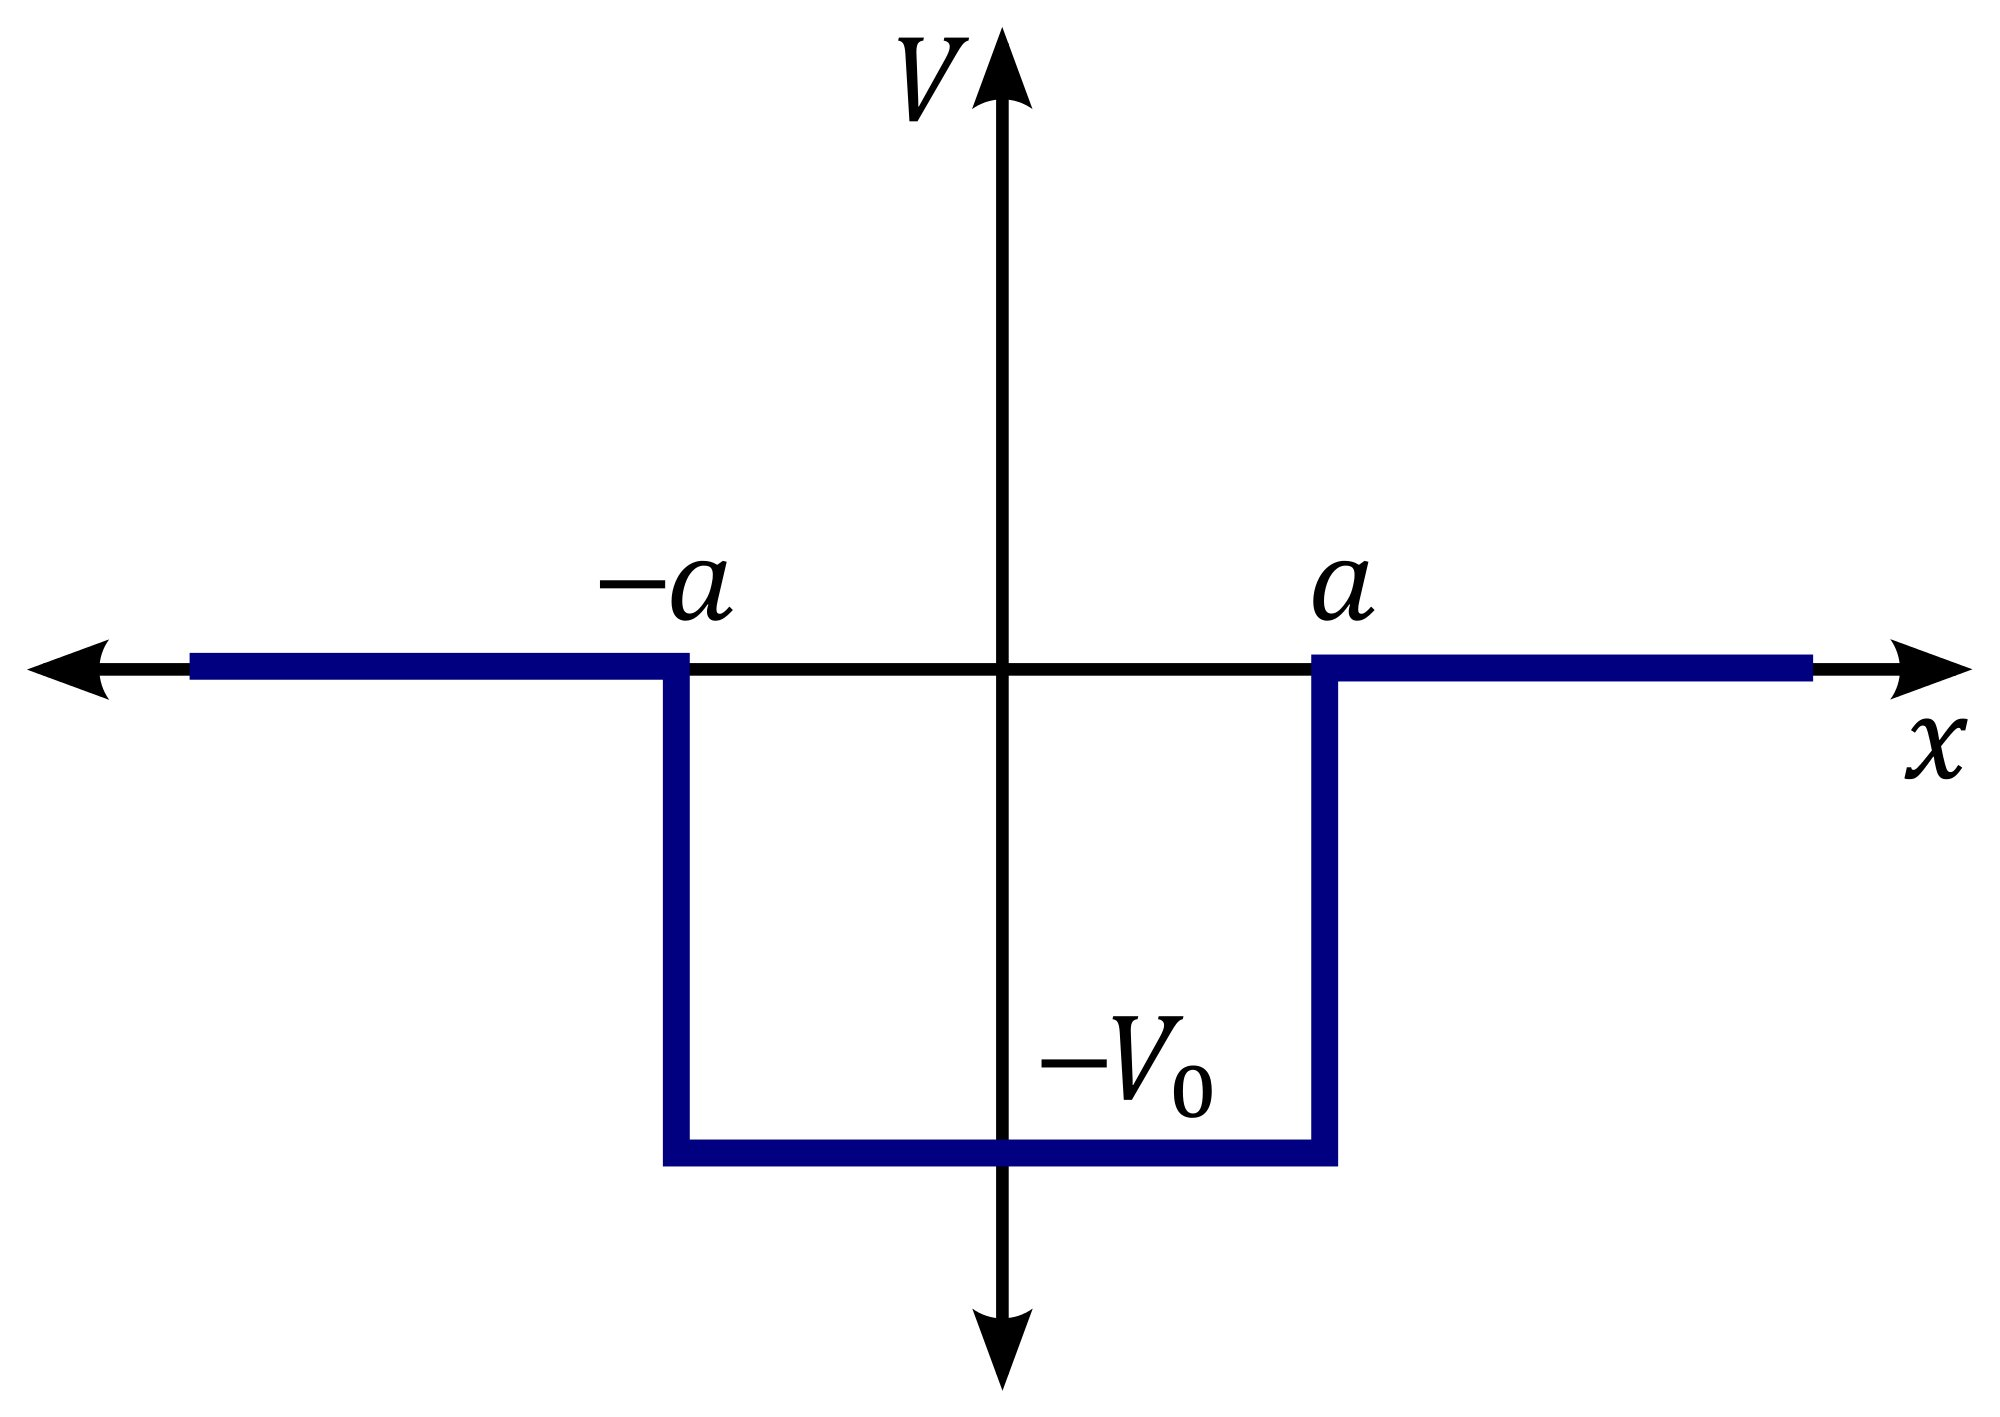
\includegraphics[scale=0.09]{FSW.jpg}
    \end{center}

\end{frame}
\begin{frame}{The Finite Square Well}
    The Hilbert space for the finite square well can be taken to be
    $L^2(\mathbb{R})$, and
    the Hamiltonian for the finite square well is 
    \[
        \hat{H}(x) =
        \begin{cases}
            \frac{-\hbar^2}{2m}\frac{d^2}{dx^2} - V_0& \text{if } x\in[-a,a]\\
            \frac{-\hbar^2}{2m}\frac{d^2}{dx^2} &\text{else}
        \end{cases}
    \]

    The goal is to find the \em allowed energies \em for this system. To do so,
    we need to find the spectrum of $\hat{H}$.
\end{frame}

\begin{frame}{The Finite Square Well: Results}
    First pass: solve $\hat{H}\psi = E\psi$ to find eigenvalues.
    As it turns out, this splits into two cases: $V_0<E<0$ and $E>0$.
    \begin{result}
        \begin{itemize}
            \item For $V_0<E<0$, the solutions are of the form
    \[
    \psi(x) =
    \begin{cases}
        C_1e^{\sqrt{\epsilon}x}& \text{if } x\in(-\infty,-a]\\
        C_2\cos(\sqrt{v-\epsilon})& \text{if } x\in[-a,a]\\
        C_3e^{-\sqrt{\epsilon}x}& \text{if } x\in [a, \infty)
    \end{cases}
    \]
                with the condition that $
    \sqrt{\epsilon} = \sqrt{v-\epsilon}\tan(\sqrt{v-\epsilon}a)$

            \item For $E>0$, the solutions are linear combinations of
                $\psi_E(x) = C_1e^{ikx} + C_2e^{-ikx}$ for
                $k=\frac{\sqrt{2mE}}{\hbar}$.
        \end{itemize}
    \end{result}
\end{frame}

\begin{frame}{The Finite Square Well: Bound states}
    For $E<V_0$, we find a finite discrete set of allowed energies.
    \begin{center}
    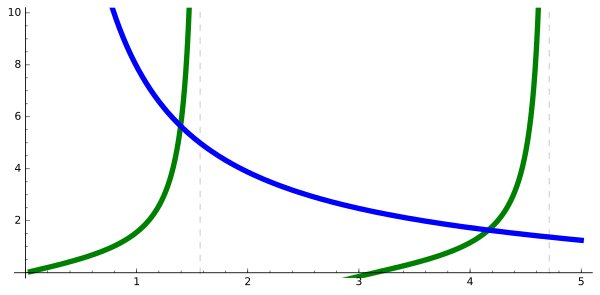
\includegraphics[scale=0.4]{transcendental_solutions}
    \end{center}
    $\sqrt{\epsilon} = \sqrt{v-\epsilon}\tan(\sqrt{v-\epsilon}a)$
\end{frame}


\begin{frame}{The Finite Square Well: Bound States(Cot'd)}
    \begin{center}
    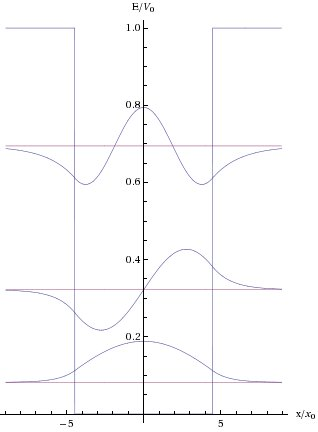
\includegraphics[scale=0.4]{FSW_soln}
    \end{center}
\end{frame}

\begin{frame}{The Finite Square Well: Spectral Partitions}
    Each bound state corresponds to an energy in the point spectrum
    $\sigma_P(\hat{H})$, and each free state corresponds to an energy in the
    approximate point spectrum $\sigma_{AP}(\hat{H})$.

    \begin{proof}
        For $E>0$, let $\psi$ solve $\hat{H}\psi=E\psi$, and define a sequence
        of functions
        \[
            \psi_n(x) = \psi *
            \begin{cases}
                0 & |x| \geq n+1\\
                1 & |x| \leq n \\
                \chi_{[0,\frac{1}{3}]}(-x-n) & -(n+1)<x<-n\\
                \chi_{[0,\frac{1}{3}]}(x-n) & n<x<n+1
            \end{cases}
            \]
        Then, it can be shown that
        $lim_{n\to\infty}\frac{||(\hat{H}-EI)\psi_n||}{||\psi_n||} = 0$.
    \end{proof}
\end{frame}

\begin{frame}{The Finite Square Well: Projection-Valued Measure}
    For this slide, $E$ will represent an element of the spectrum of $\hat{H}$,
    and $F$ will be a projection-valued measure.

    \begin{itemize}
        \item For the point spectrum, 
    \[
        dF(E) = P_E
    \]
    where $P_E$ is the orthogonal
    projection onto the one dimensional subspace of the state with energy $E$.

\item For the approximate point spectrum, one can interpret $dF(E)$ to be a
    projection onto the two dimensional subspace spanned by the "states"
    \[
        \begin{aligned}
            \psi_{E}(x) &= e^{-ikx} \\
            \psi_{E}(x) &= e^{ikx}
        \end{aligned}
    \]
    \end{itemize}
\end{frame}

\begin{frame}{The Finite Square Well: Projection-Valued Measure (Cot'd)}
    Problem:
    \[
        \begin{aligned}
            \psi_{E}(x) &= e^{-ikx} \\
            \psi_{E}(x) &= e^{ikx}
        \end{aligned}
    \]
    is not in $L^2(\mathbb{R})$!

    \pause

    This is because $\mu(E) = 0$...

    \pause

    For a set of positive measure (e.g. an interval of energies), we get
    infinitely many frequencies to work with, and can build a square-integrable
    function from them!

    \begin{example}
        For an interval of energies $k\in[1,2]$, the state
        \[
            \psi(x) = \int_{[1,2]}\chi_{[1,2]}(x)e^{ikx}dk
            \]
        is a square-integrable solution!
    \end{example}
\end{frame}
\begin{frame}{The Finite Square Well: Direct Integral}
    The spectrum of $\hat{H}$ is $\sigma(\hat{H}) = {E_n}\cup(0,\infty)$ for
    some finite set of allowed bound energies $E_n$.

    The measure on the point spectrum is the counting measure, so that part of
    the integral becomes
    \[
        \int_{\sigma_P(\hat{H})}^{\oplus}\textbf{H}_{E}d\mu(E) =
        \oplus_{i=1}^{n} \textbf{H}_{E}
    \]
Where $\textbf{H}_E$ is the one dimensional subspace of the state with energy
    $E$.
\end{frame}

\begin{frame}{The Finite Square Well: Direct Integral}
    The measure on the approximate point spectrum is more mysterious, but the
    integrand $\textbf{H}_E$ can be shown to be the two-dimensional subspace of
    complex exponentials $e^{ikx}$ and $e^{-ikx}$.

    Thus, the Hilbert space for which $\hat{H}$ acts as multiplication is
    \[
        \oplus_{i=1}^n \textbf{H}_{E_n} \oplus
        \int_{\sigma_{AP}(\hat{H})}^{\oplus} H_Ed\mu(E)
    \]
\end{frame}

\begin{frame}{Conclusions}
    \begin{itemize}
        \item The spectral theorem still works in infinite dimensions.
        \item Infinite dimensions potentially leads to a continuous spectrum.
        \item This is fixed by introducing an integral across the more
            generalized eigenspaces, either on projections (PVM) or on the space
            itself (DI).
        \item Spectral partitions help with understanding which parts of the
            spectrum will be continuous or not.
        \item These formulations provide a new perspective on some key results
            in quantum mechanics
    \end{itemize}

\end{frame}

\begin{frame}
\begin{center}

\includegraphics[scale=0.5]{dead_alive_cat}
\end{center}
\begin{center}
\emph{\textbf{  Special thanks to Dr. Gaebler,\\
                The Hillsdale College Mathematics Department,\\
                And viewers like you!}}
\end{center}
\end{frame}
\end{document}
\end{document}
